\documentclass{llncs}
\pagestyle{plain}

%\usepackage[latin9]{inputenc}
%\usepackage[T1]{fontenc}
\usepackage{float}
\usepackage{wrapfig}
\usepackage{amsmath}
\usepackage{amssymb}
\usepackage{graphicx}
\usepackage{subcaption}
\captionsetup{compatibility=false}
% \usepackage{esint}
\usepackage{array}
\usepackage{epstopdf}
\usepackage{placeins}
\usepackage{url}
\usepackage{tikz}
\usepackage{calc}
\usetikzlibrary{positioning, arrows.meta,calc}
%%%%%%%%%%%%%%%%%%%%%%%%%%%%%%%
%%%%%%%%%%%%%%%%%%%%%%%%%%%%%%%







%\usepackage{amsmath, amsthm, amssymb, amsfonts}
%\newtheorem{theorem}{Theorem}
%\newtheorem{lemma}{Lemma}
%\newtheorem{corollary}{Corollary}
%\theoremstyle{definition}
%\newtheorem{definition}{Definition}



\newcommand{\ReLU}{\mathrm{ReLU}}



\title{I Compensate, therefore I Am \\ (accurate for DNN verification)}
\date{}

\begin{document}

\maketitle

\begin{abstract}
  Deep Neural Networks (DNNs) verification is now a mature research field, with many methodologies and tools to verify formaly  that they are correct, with an annual competition to compare them, etc. Formally, the question is, given a DNN and a property to check, does the property hold over a set of inputs of the DNN. This allows e.g. to check local robustness around an input $I$, by checking that the i-th output neuron has the largest weight among all output neurons uniformly over a neighbourhood around $I$.
  In the most recent years, the focus has been on combining several of these efficient techniques (branch and bound, multi neuron encoding, MILP encoding, ...) to optimize speed/accuracy trade-offs. While some relatively large DNNs (tens of thousands of neurons) can be checked very efficiently with modern tools, some DNNs are still challenging to address with efficient algorithms, even small ReLU DNNs with hundreds of neurons, showing the need for new methodologies.

  In this paper, we analyze efficient algorithms to verify ReLU DNNs, based on abstractions (DeepPoly, Linear Programing, PRIMA, different version of Crown), and uncover the main reason for the loss of accuracy, namely {\em compensations}. Intuitively, a compensation happens when there are 2 paths between the same pair of neurons, one path with positive and one path with negative (product of) weights, which therefore (partly) compensate each other. It is however hard to compute exactly by how much is the compensation due to the ReLU activation functions. Based on this finding, we propose a novel methodology to obtain interesting trade-offs in terms of speed/accuracy, using many queries with few 'open' ReLU nodes (for which both linear modes are considered), rather than the usual few queries with potentially many 'open' ReLU nodes. These promising results open up many different applications of the concept of compensating paths in the field of verification of DNNs.
\end{abstract}


\section{Introduction}


Complexity


This paper does not focuss on producing the most efficient tool, and we did not spend engeenierial effort to optimize it. The focus is instead on the novel notion of compensation, the associated methodology and its evaluation. For instance, our implementation is fully in Python, with uncompetitive runtime for our DeepPoly implementation ($\approx 100$ slower than in $\beta$-CROWN). Still, evaluation of the methodology versus even the most efficient tools reveal a lot of potential for the notion of compensation, opening up several opportunities for applying it in different contexts of DNN verification.






\section{Background}

We follow some notions in PRIMA's and Beta-Crown's papers: we use lower case Latin for scalars, bold for vectors
$\boldsymbol{z}$, capitalized bold for matrices $\boldsymbol{W}$. In this paper, we will not use tensors with a dimension higher than matrices: those will be flattened.




\subsection{Neural Network and Verification}

% testtesttesttest

We focus on full-connected neural network. The network has weights and bias to send the input to output along hidden layers. In formula, the input layer of a neural network is a vector $\boldsymbol{x}$ in $\mathbb{R}^{d_0}$, and the $i$-th hidden layer  is a vector in $\mathbb{R}^{d_i}$, and the output layer is a vector in $\mathbb{R}^{d'}$ or a scale. The weights, bias and activation functions decide propagate the from previous to the next layer. In formula, from layer $l_{i-1}$ to layer $l_{i}$, the weight $\boldsymbol{W}^i$ is matrix of $d_i\times d_{i-1}$, the bias is a vector $\boldsymbol{b}^i$ in $\mathbb{R}^{d_i}$, and the activation function is $\sigma$, then  if the $i-1$-th layer is $\hat{\boldsymbol{z}}^{(i-1)}$, then the value of $i$-th layer is computed by: \begin{align*}
	{\boldsymbol{z}}^{i} &= \boldsymbol{W}^i\cdot \hat{\boldsymbol{z}}^{(i-1)}+ \boldsymbol{b}^i\\
	\hat{\boldsymbol{z}}^{i}(n) &= \sigma({\boldsymbol{z}}^i(n)).
\end{align*} The vector $\hat{\boldsymbol{z}}$ is called post-activation values, and $\boldsymbol{z}$ is called pre-activation values, and $\boldsymbol{z}^{(i)}_j$ is used to call the $j$-th neuron in the $i$-th layer. In our style, we also call neurons \emph{nodes} and use $a,b,c,d$ to denote them. We use $W_{ab}$ to denote the weight from neuron $b$ to $a$. We use $\boldsymbol{x}$ to denote the vector of input and  $f(\boldsymbol{x})$ to denote the output.


The verification problem is to determine whether the output of a neural network will be affected under small perturbations to the input. In formula, if we use a distance $d$, and if the $\boldsymbol{x}_0$ is a ordinary input, then the considered domain $\mathcal{D}=\{x: d(\boldsymbol{x},\boldsymbol{x}_0)<\varepsilon\}$ where $\varepsilon$ is the parameter measuring the size of perturbation. And the problem will be \begin{align*}
	\forall \boldsymbol{x}\in\mathcal{D} \   f(\boldsymbol{x}) = f(\boldsymbol{x}_0).
\end{align*} In some cases, the output is a vector but the aim to get the label of dimension with the minimal value. In this case, the problem can be written as:\begin{align*}
\forall \boldsymbol{x} \in\mathcal{D} \  \min f(\boldsymbol{x}) = \min f(\boldsymbol{x}_0)
\end{align*}

If so, the question of verification can turn to the following optimization question: \begin{align*}
	\min f(\boldsymbol{x}) \ s.t. {\boldsymbol{z}}^{i} &= \boldsymbol{W}^i\cdot \hat{\boldsymbol{z}}^{(i-1)}+ b^i\\
	\hat{\boldsymbol{z}}^{i}(n) &= \sigma({\boldsymbol{z}}^i(n)), \boldsymbol{x}\in\mathcal{D}.
\end{align*}

In this paper, we only consider $\ReLU$ function as the activation function: $\sigma(a)=\ReLU(a)=\max(0,a)$. We will consider $L^{\infty}$ norm, that is $$d(\boldsymbol{x},\boldsymbol{x}_0)=\max |\boldsymbol{x}(n)-\boldsymbol{x}_0(n)|,$$ the max value of distance of each dimension.



\subsection{MILP formation of $\ReLU$ functions}

In literature, many methods have been used to approximate $\ReLU$ functions. One of them is MILP (or MIP, Mixed Integer Linear Programming).

For a activation $x=\ReLU(y)$, if we already know $y's$ rough upper and lower bounds $u,l$, then if $u>0$ and $l<0$, we call $y$ is unstable; otherwise, $y$ is stable. In practice, stable node is easier because $\ReLU$ function becomes a linear function on this node. The key problem is to deal with unstable nodes.

In literature, if $x=\ReLU(y)$, and $y$ is unstable, then this function can be formulated in MILP with one integer variable $a$ valued in ${0,1}$ (i.e., a binary variable) by:

\vspace*{-4ex}

\begin{align*}
	&x \geq 0, \ 
	x \geq y-l\cdot (1-a)\\
	&x \leq y,\ 
	x \leq u\cdot a
\end{align*} 

MILP becomes one of standard methods to compute the lower bounds and upper bounds of neurons in a pure $\ReLU$ activation network. Combining with the discussion from previous subsection, the verification problem is equivalent to an MILP optimization problem.

However, the cost of optimization of an MILP model is very expensive, especially when the number of binaries increases: solving MILPs are NP-hard, and often needs exponential time to solve it. A typical relaxation is to change the binary variable $a$ to a continue variable, then it will be equivalent to the standard triangle LP model for $\ReLU$ function.

Our strategy is to restrict the number of binary variables, and this will definitely lose accuracy of results.  The key problem is how to use fewer binary variables to get more accuracy. That is, to choose which node to be binary, and which not.

\begin{definition}
	1. For a full-connected DNN with $\ReLU$ activation, to compute the upper or lower bound of a node (in a hidden layer or output layer), its MILP model is formulated as follows: 
	
	(1) For every node in the input layer $a$, set a $z_a$ variable with the same input interval: $l_a\leq z_a\leq u_a$
	
	(2) For each hidden layer $l^i$, set two variables , $z_c,\hat{z}_c$ for each node $c$ in this layer for pre-activation and post-activation. 
	
	The constraints for pre-activation $z_a$ is the natural linear equation by the network. 	$$z_c=\sum_{d\in l^{i-1}} W^i_{cd} z_d+b^i_c.$$
	
	
	The constraints for $\hat{z}_a$ is defined by the standard MILP formulation mentioned above with known upper bound and lower bound as parameters.
	
	\vspace*{1ex}
	
	Since we only consider such MILP models, so when we say an MILP model, it is for a full-connected DNN with $\ReLU$ activation. 
	
	2. In an MILP model, we say a $\ReLU$ node is open, if the binary variable corresponds to this function is still an binary variable; otherwise, it is relaxed as a continue variable. 
\end{definition}

We aim is to find an algorithm, to decide which nodes should be opened such that we can have more accuracy.

\section{Compensate, Diamond and Node Chosen}

In this section, we will explore the key factor for the loss of accuracy in our LP/MILP models: \emph{compensating pair}. And we will develop a process of open node chosen by the principle of \emph{Compensating Pairs}. 



\subsection{Compensating pair}

The basic mode of compensating pair is as follows:

\vspace*{2ex}

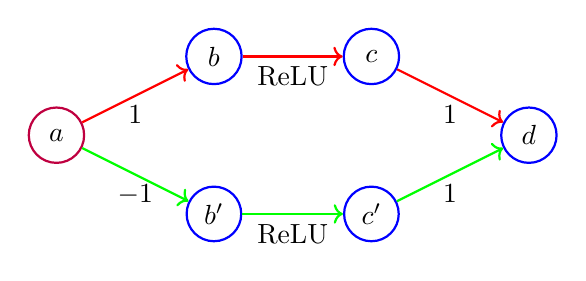
\begin{tikzpicture}
	\node[circle, draw= purple, thick, minimum width = 20,
	minimum height = 20] (input1) {$a$};

	
	% Hidden layers
	\node[circle, draw= blue, thick, minimum width = 20,
	minimum height = 20] (hidden1) at ($(input1) + (2,1)$) {$b$};
	\node[circle, draw= blue, thick] (hidden2) at ($(input1) + (2,-1)$) {$b'$};
	
	\node[circle, draw= blue, thick, minimum width = 20,
	minimum height = 20] (hidden3) at ($(input1) + (4,1)$){$c$};
	\node[circle, draw= blue, thick] (hidden4) at ($(input1) + (4,-1)$) {$c'$};
	
	% Output layer
	\node[circle, draw= blue, thick, minimum width = 20,
	minimum height = 20] (output) at ($(input1) + (6,0)$){$d$};
	
	% Connections
	\draw[->,thick,draw= red] (input1) -- (hidden1) node[midway, below] {$1$};
	\draw[->,thick,draw= green] (input1) -- (hidden2)node[midway, below] {$-1$};
	
	\draw[->,thick,draw= red] (hidden1) -- (hidden3) node[midway, below] {$\ReLU$};
	\draw[->,thick,draw= green] (hidden2) -- (hidden4) node[midway, below] {$\ReLU$};
	
	\draw[->,thick,draw= red] (hidden3) -- (output)node[midway, below] {$1$};
	\draw[->,thick,draw= green] (hidden4) -- (output)node[midway, below] {$1$};
\end{tikzpicture}

\vspace*{2ex}

In this figure, $a$ is the input neuron; $bc,b'c'$ are nodes in the hidden layer, ($b,b'$ are pre-activation and $c,c'$ are post activation); and $d$ is the unique output neuron. The numbers next to the arrows are the weights. So, $W_{ba}=1$ and $W_{b'a}=-1$, $W_{dc}=W_{dc'}=1$. The pair of these two paths, $a$ to $bc$ to $d$, and $a$ to $b'c'$ to $d$, is a so called \emph{Compensating Pair}. Because its shape looks like a diamond, it is also called a Diamond. The characteristic is that, the products of all weights in the paths, have two different signs: along $bc$, the product is (strictly) positive, while along $b'c'$, the product is (strictly) negative. 

The existence of compensating pairs is key reason why simple approximation like LP or Interval Arithmetic cannot get the exact upper and lower bounds. If both pairs are negative or positive, LP or even Interval Arithmetic will get the exact values of lower and upper bounds.


To explain why, suppose we have another input node $a'$, such that both $a$ and $a'$ has an input interval $[0,1]$, but the weight from $a'$ to $b$ or $b'$ are both $1$. Then both $b$ will have an interval $[0,2]$ and $b'$ will have an interval $[-1,1]$. More importantly, in LP formulation, $c$ will be $b$ but $c'$ will be $0.5(b')+0.5$. The upper bound of $d$ will be $c+c'$, and hence $b+0.5(b')+0.5$, and hence $a+a'+0.5a'-0.5a'+0.5=0.5a+1.5a'+0.5$. And this will leads to a upper bound $2.5$ but this is not exact.

\vspace*{2ex}
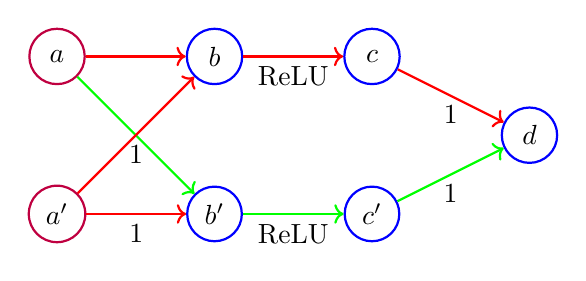
\begin{tikzpicture}
	\node[circle, draw= purple, thick, minimum width = 20,
	minimum height = 20] (input1) {$a$};
	
	\node[circle, draw= purple, thick, minimum width = 20,
	minimum height = 20] (input2) at ($(input1) + (0,-2)$) {$a'$};
	
	
	% Hidden layers
	\node[circle, draw= blue, thick, minimum width = 20,
	minimum height = 20] (hidden1) at ($(input1) + (2,0)$) {$b$};
	\node[circle, draw= blue, thick] (hidden2) at ($(input1) + (2,-2)$) {$b'$};
	
	\node[circle, draw= blue, thick, minimum width = 20,
	minimum height = 20] (hidden3) at ($(input1) + (4,0)$){$c$};
	\node[circle, draw= blue, thick] (hidden4) at ($(input1) + (4,-2)$) {$c'$};
	
	% Output layer
	\node[circle, draw= blue, thick, minimum width = 20,
	minimum height = 20] (output) at ($(input1) + (6,-1)$){$d$};
	
	% Connections
	\draw[->,thick,draw= red] (input1) -- (hidden1);
	\draw[->,thick,draw= green] (input1) -- (hidden2);
	
	\draw[->,thick,draw= red] (input2) -- (hidden1) node[midway, below] {$1$};
	\draw[->,thick,draw= red] (input2) -- (hidden2)node[midway, below] {$1$};
	
	\draw[->,thick,draw= red] (hidden1) -- (hidden3) node[midway, below] {$\ReLU$};
	\draw[->,thick,draw= green] (hidden2) -- (hidden4) node[midway, below] {$\ReLU$};
	
	\draw[->,thick,draw= red] (hidden3) -- (output)node[midway, below] {$1$};
	\draw[->,thick,draw= green] (hidden4) -- (output)node[midway, below] {$1$};
\end{tikzpicture}
\vspace*{2ex}

The general formal definition of compensating pair is as follows:

\begin{definition} In a full-connected network with $\ReLU$ as activation function:
	
	1. A path is a sequence of nodes $\langle a,b,c,d,e,\cdots\rangle$ of nodes that goes consecutively through each layer. We call the first node source node and the last node target node.  
	
	2. The \emph{Value} of a path is the product of of weights along the path (with sign): for a path $\langle a,b,c,d,e,\cdots\rangle$, its values is $$V = W_{ba}\cdot W_{cb}\cdot W_{dc}\cdot W_{ed}\cdot \cdots$$
	
	3. A \emph{Compensating Pair} is a pair of paths with the same source node and target node, such that the two paths have no common node, and the values of two paths have opposite signs (one is strictly positive and another is strictly negative).
	
	We also use \emph{Diamond} to call a compensating pair in the network.
\end{definition}


The following theorem shows the role of compensating pairs in the computation:

\begin{theorem}[No Diamond Theorem, part 1]
	For a full-connected network with $\ReLU$ as the unique activation function, if there is no Diamond, then for any method/approximation that at least as accurate as Interval Arithmetic, it can get the exact upper and lower bounds of all output nodes and all hidden nodes.
\end{theorem}

Of course, in practice, it is very unlike to have a network without any Diamond. Therefore, the second theorem is more important in practice.

\begin{theorem}[No Diamond Theorem, part 2]
	For a full-connected network with $\ReLU$ as the unique activation function. If we open all nodes that occurs in a compensating pair path, then the we can get the exactly bounds.
\end{theorem}

The proofs of above theorems are in the Appendix.

\subsection{Paths and Open Nodes Chosen}

In this subsection, we will introduce the method to choose open nodes for MILP model by considering compensating pairs.

Based on No Diamond Theorem, for a target node, in its MILP model, if we open all nodes in compensating pairs, then we can get the exact values of upper and lower bound of the target node. However, in practice, this is still too expensive because we will still need to open too many nodes. So we can only choose a limited number of compensating pairs and nodes. This is by setting a parameter $O$ such that the process only choose at most $O$ many nodes to open. Therefore, in this subsection, we will introduce the process of open node chosen: given a target node, choose up to $O$ many nodes to open.


Basically, we do the process of open nodes chosen for one target node each time, that is, receive one target node (and other data) as input each time. But in principle, we can develop a method receive more than one nodes as input. But in our experiences, this does not work well.  

This process is not the unique method but the most natural way to choose open nodes. We introduce it in three steps from the simplest case to more complex case.

\subsubsection*{Value of a pair}


For a compensating pair, if $V_1,V_2$ are the values of two paths, then the value of this compensating pair is defined by: $V=\min(|V_1|,|V_2|)$.


\subsection*{Case: Source node fixed}

The simplest case is when we only consider compensating pairs with a fixed source node. 

In this case, the process is very simple: enumerate all compensating pairs, and then sort them by their values. Finally, from the first to the last compensating pair, pick all unstable nodes in its two paths except the target and source nodes into the list of open nodes, until $O$ many open nodes. 

%\subsubsection*{Sort all paths by values}
%
%The first step is to sort all paths by their values and divide paths into two groups, a group of paths with positive values and a group of paths with negative values.
%
%Since we have set a bound $O$ for open nodes, we will store  a fixed number of path for each group.
%
%\subsubsection*{Sort pairs by values}
%
%The second step is to sort all pairs by their values. Enumerate paths from the positive group and the negative group one by one and put the pairs obtained into a new list of pairs. Then sort all pair by their values from largest to the smallest: recall that the value of a pair $\langle P_1,P_2\rangle$ is $\min(|V_1|,|V_2|)$.
%
%\subsubsection*{Choosing nodes}
%
%The third step is to choose nodes from the list of pairs. According to the sorted list of pairs, enumerate pair one by one; for each pair, pick the nodes unstable in the two paths except the source and target node into the open node list. Repeat this process until $O$ nodes chosen or reach the end of the list.
%
%\subsubsection*{Pseudocode}
%
%The following needs a chart of pseudo-code
%
%\vspace*{1ex}
%
%1. Enumerate all path from the fixed source node to the target node. 
%
%2. For each path, compute its weight, that is the products of all $W_{aa'}$ along the path.
%
%3. Divide all paths into two group: positive paths and negative paths.
%
%4. Pair positive paths and negative paths from those with larger absolute values to smaller. 
%
%5. For each pair, its value is the min of the weight positive paths and absolute negative values.
%
%6. From pairs with larger values to smaller, pick path one by one, and check all intermediate nodes (nodes except source and target) of each path, and if any of them is unstable ($u>0$ and $l<0$), then open this node. 
%
%7. Repeat 6 until choosing sufficiently many nodes.
%





\subsection*{Case: Source nodes in one layer}

The more general case is when the source node can be any node in a fixed layer. In this case, the process is very similar to previous case, except the value of a pair.

In this case, for a pair $P_1,P_2$ with values $V_1,V_2$ with the source node $a$, its value is $\min(|V_1|,|V_2|)\times \text{upper bound of } a$.

%\subsubsection*{Pseudocode}
%
%The following needs a chart of pseudo-code
%
%\vspace*{1ex}
%
%1. Enumerate all path from the fixed source node to the target node. 
%
%2. For each path, compute its weight, that is the products of all $W_{aa'}$ along the path.
%
%3. Divide all paths into two group: positive paths and negative paths.
%
%4. Pair positive paths and negative paths from those with larger absolute values to smaller. 
%
%5. For each pair, its value is the min of the weight positive paths and absolute negative values, times the upper bound (at least 0) of the source node.
%
%6. From pairs with larger values to smaller, pick path one by one, and check all intermediate nodes (nodes except source and target) of each path, and if any of them is unstable ($u>0$ and $l<0$), then open this node. 
%
%7. Repeat 6 until choosing sufficiently many nodes.







\subsection*{Case: Source nodes in different layers}

The general case is that when the location of source nodes can be in different layers. This case is much more complex, because the scale level of values of paths from different layers are very different: usually a weight will be very small since every layer has a large number of nodes, therefore values of longer paths are products of more small numbers, and is definitely much smaller. If we sort all compensating pairs from different layers directly, then a very long initial segment of this list will be occupied by compensating pairs with the shortest length. Therefore, we need use some scale factors when comparing values of compensating pairs of different length.

In our experiments, we only consider the paths of length 3 (the source node is 2 layers before) and length 4 (the source node is 3 layers before). We will dynamically adjust the values during the process of node chosen.

\subsubsection*{Pseudocode}

The following needs a chart of pseudo-code

\vspace*{1ex}

1. Generate the two lists of pairs sorted by their values for source nodes in 2 layers before the target node and 3 layers before separately as in the previous case.

2. Enumerate pair from two lists one by one by their values and pick nodes as previous case. When comparing the values between pairs of length 4 and pairs of length 3, multiply the numbers of nodes in 1 layer before to the value of pair of length 4.

In formula, when the target node is in layer $L$, for a pair $P_3$ of length 3 with value $V_3$ and a pair $P_4$ of length 4 with value $V_4$, if we have chosen $N$ nodes in layer $L-1$. Then the adjusted values for $P_3$ and $P_4$ are: $$V_3, N\cdot V_4.$$ Then we pick the next pair by the adjust value in two lists.

3. Repeat 2 until choosing sufficiently many nodes.


\section{Verification Framework}



%Our experiments are carried by different version codes, and the global process has been changed. 

We explain the framework in 4 subsections: precomputation, process for one image, process for one node, and global process.

\subsection{Process for one image}

The basic unit of running is image: all parameters will be reset when one image is finished.

The process for one image is clear: compute the upper and lower bounds of nodes layer by layer to the output layer. 

Suppose we have reached a new layer $l_i$ and have upper and lower bounds of all nodes in previous layers. Then we will compute bounds of every node in $l_i$ in parallel using the data of bounds of previous nodes. The method is to build and optimize an MILP model.

Some parameters may be changed during layers. Among all parameters, two groups are the most important: numbers of open nodes and local timeout parameters. Here, \emph{local} is opposite to \emph{global}. We have global timeout parameters for images and the whole running. Local timeout are used in one layer, one node, one model, or one loop in the optimization for a model.

In one layer, in principle, running for nodes are in principle independent and can be done in parallel. In our experiments, some local parameters will be adjusted from nodes to nodes.

\subsection{Precomputation}

The open node chosen is the key part of the whole framework, and it will cost two much time without precomputation because we must do open node chosen for every node. 

The precomputation corresponds to the simplest case: source node fixed. We will compute and store a limited number of paths with highest (absolute) values before running any image. This does not rely on other parameters or results(bounds).

Before build an MILP model and when choosing open nodes list,  the program will read the reference data combining with the data of bounds to continue the computation of open nodes. This will use much less time.


\subsection{Process for one node}

For one node, we will build the MILP model for it.

The most important parameter is the number $O$ mentioned in last section:  the number of open nodes. When the program creates a model for a node, we will read this parameter to decide how many nodes to open in this model. This parameter can change during the running of an image by the mechanic of the code.


Another group of parameters is for the optimization of models. 

The optimization of a model is carrying by loops. For each loop, the model will do optimization by a timeout and observe the result. If it gets improvement, then continue the loop until the optimize bounds or the longer timeout. Otherwise it will give up optimization and store the best bounds obtained so far.  

During the loop of optimization, parameters might be changed and the model may be rebuild by the new parameter.


\subsection{Global Process}

In the newest version, we do images by batches for 100 images each. For each batch, the running consists of three turns, very fast turn, fast turn and slow turn.

In the very fast turn, it will run DeepPoly for all images to get a preliminary bounds for all nodes and verify the easiest images. Images verified and images with false predication will be deleted from the image list.

Then sort all remain images by the size of uncertainty of DeepPoly from smaller to larger. The fast turn is to run the images from the smaller side to larger side until consecutive two images cannot be verified. All remain images and images tried but not verified will be put into the next list. And then run the list with parameters for slow turn.

%\subsubsection*{Run one image}
%
%In the very fast turn, we use DeepPoly. So, all discussion below only consider fast and slow turns.
%
%An image is the basic unit in the running. The running is carrying layer by layer. The bounds obtained in previous layer will be used to build the model for the next layer, till the output layer.
%
%Some parameters may be changed during layers. Among all parameters, two groups are the most important: numbers of open nodes and local timeout parameters. Here, \emph{local} is opposite to \emph{global}. We have global timeout parameters for images and the whole running. Local timeout are used in one layer, one node, one model, or one loop in the optimization for a model.
%
%In one layer, in principle, running for nodes are in principle independent and can be done in parallel. In our experiments, some local parameters will be adjusted from nodes to nodes.


%\subsubsection*{Create Models}
%
%The most important parameter is the number $O$ mentioned in last section:  the number of open nodes. When the program creates a model for a node, we will read this parameter to decide how many nodes to open in this model. This parameter can change during the running of an image by the mechanic of the code.
%
%\subsubsection*{Optimization for a node}
%
%Another group of parameters is for the optimization of models. 
%
%The optimization of a model is carrying by loops. For each loop, the model will do optimization by a timeout and observe the result. If it gets improvement, then continue the loop until the optimize bounds or the longer timeout. Otherwise it will give up optimization and store the best bounds obtained so far.  
%
%During the loop of optimization, parameters might be changed and the model may be rebuild by the new parameter.

\subsubsection*{Other Setting}

In our experiments, we have not used PGD-attack to rule out images. In principle, there is no obstacle to use PGD-attack.



\section{Experimental Evaluation}

The neural network certification benchmarks for fully connected networks were run on a 32 core
GHz Intel with 256 GB of main memory. We use Gurobi 9.52 for solving MILP and LP problems


We used MNIST image datasets for our experiments. MNIST contains grayscale images of size 28 × 28 pixels. For our evaluation, we chose the first
1000 images from the test set of each dataset.

Each data example is associated with an $L^\infty$ norm $\varepsilon$ and a target label
for verification.

\subsection{Experiments about Node Chosen}

The first group of experiments is to test the direct effect of node chosen by compensating pair, comparing to random chosen. We use the average of uncertainty of all nodes in a layer to measure the effect of node chosen: for a node $a$, its uncertainty $UN(a) = UB(a)-LB(a)$, and the average uncertainty of a layer $l$ is $$UN(l) = \dfrac{\sum_{a\in l}UN(a)}{|l|}.$$

The test neural network is MNIST fully-connected $6\times 100$, and the test image is the image 59 in the standard MNIST image database. This image can have more unstable nodes in each layer.

\subsubsection*{Node chosen in second hidden layer}

The following table shows the average uncertainty of the second hidden layer when choosing different numbers of open nodes by random or by compensating pairs.


\subsubsection*{Node chosen in the third hidden layer}

The following table shows the average uncertainty of the third hidden layer when choosing different numbers of open nodes, by random or by compensating pairs.


\subsection{Experiments Results}

The following table is the summary of 5 experiments.


\subsection{Comparison to Incomplete Verifiers}

We compare our method to two famous verifiers (their incomplete mode): PRIMA and $\beta$-Crown on 5 typical MNIST models. Basically, our method can exceed PRIMA on both accuracy and speed, and exceed $\beta$-Crown on accuracy. 


We do tests on 5 typical MNIST models.

\section{Related Work}

\section{Conclusion}

\section*{Appendix: Proofs of No Diamond Theorem}





\end{document}


